\documentclass{article}

\usepackage[italian]{babel}
\usepackage[letterpaper,top=2cm,bottom=2cm,left=3cm,right=3cm,marginparwidth=1.75cm]{geometry}
\usepackage{amsmath}
\usepackage{graphicx}
\usepackage{subcaption}
\usepackage{textcomp}
\usepackage{ragged2e}
\usepackage[dvipsnames]{xcolor}
\usepackage{fancyhdr}
\usepackage[colorlinks=true, allcolors=blue,
            pdfauthor={Matteo Drago},
            pdftitle={Bivacco Malga Laresè di sotto},
            pdfsubject={Diario bivacchi e trekking},
            pdfkeywords={bivacco, montagna, trekking, diario}]{hyperref}

\title{\textbf{Bivacco Malga Laresè di sotto - 1774 m s.l.m}}
\author{Matteo Drago}

% ==========================================================
% Impostazioni per il logo in ogni pagina
% ==========================================================
\pagestyle{fancy}
\fancyhf{} % Pulisce tutti i campi di intestazione e piè di pagina
\fancyhead[R]{
\includegraphics[height=1.5cm]{images/toothless.jpeg}} % Posiziona il logo a destra (R) nell'intestazione
\renewcommand{\headrulewidth}{0pt} % Rimuove la linea orizzontale nell'intestazione (opzionale)


\begin{document}
\maketitle
\thispagestyle{fancy} % Aggiungi questa riga

\begin{abstract}
Questo documento raccoglie e organizza le informazioni che ho acquisito nel corso degli anni sui bivacchi, basate sulle mie esperienze dirette. Sebbene non si proponga come una guida esaustiva e perfetta, offre il minimo indispensabile per una buona vita in bivacco, con consigli pratici e diretti per chiunque desideri affrontare al meglio queste pazze ma piacevoli avventure.
\end{abstract}

\section{Il bivacco}

% ==========================================================
% Immagine a sinistra, testo a destra allineato in alto
% ==========================================================
\noindent
\begin{minipage}[t]{0.45\textwidth}
  \vspace{0pt} % forza l'allineamento in alto
  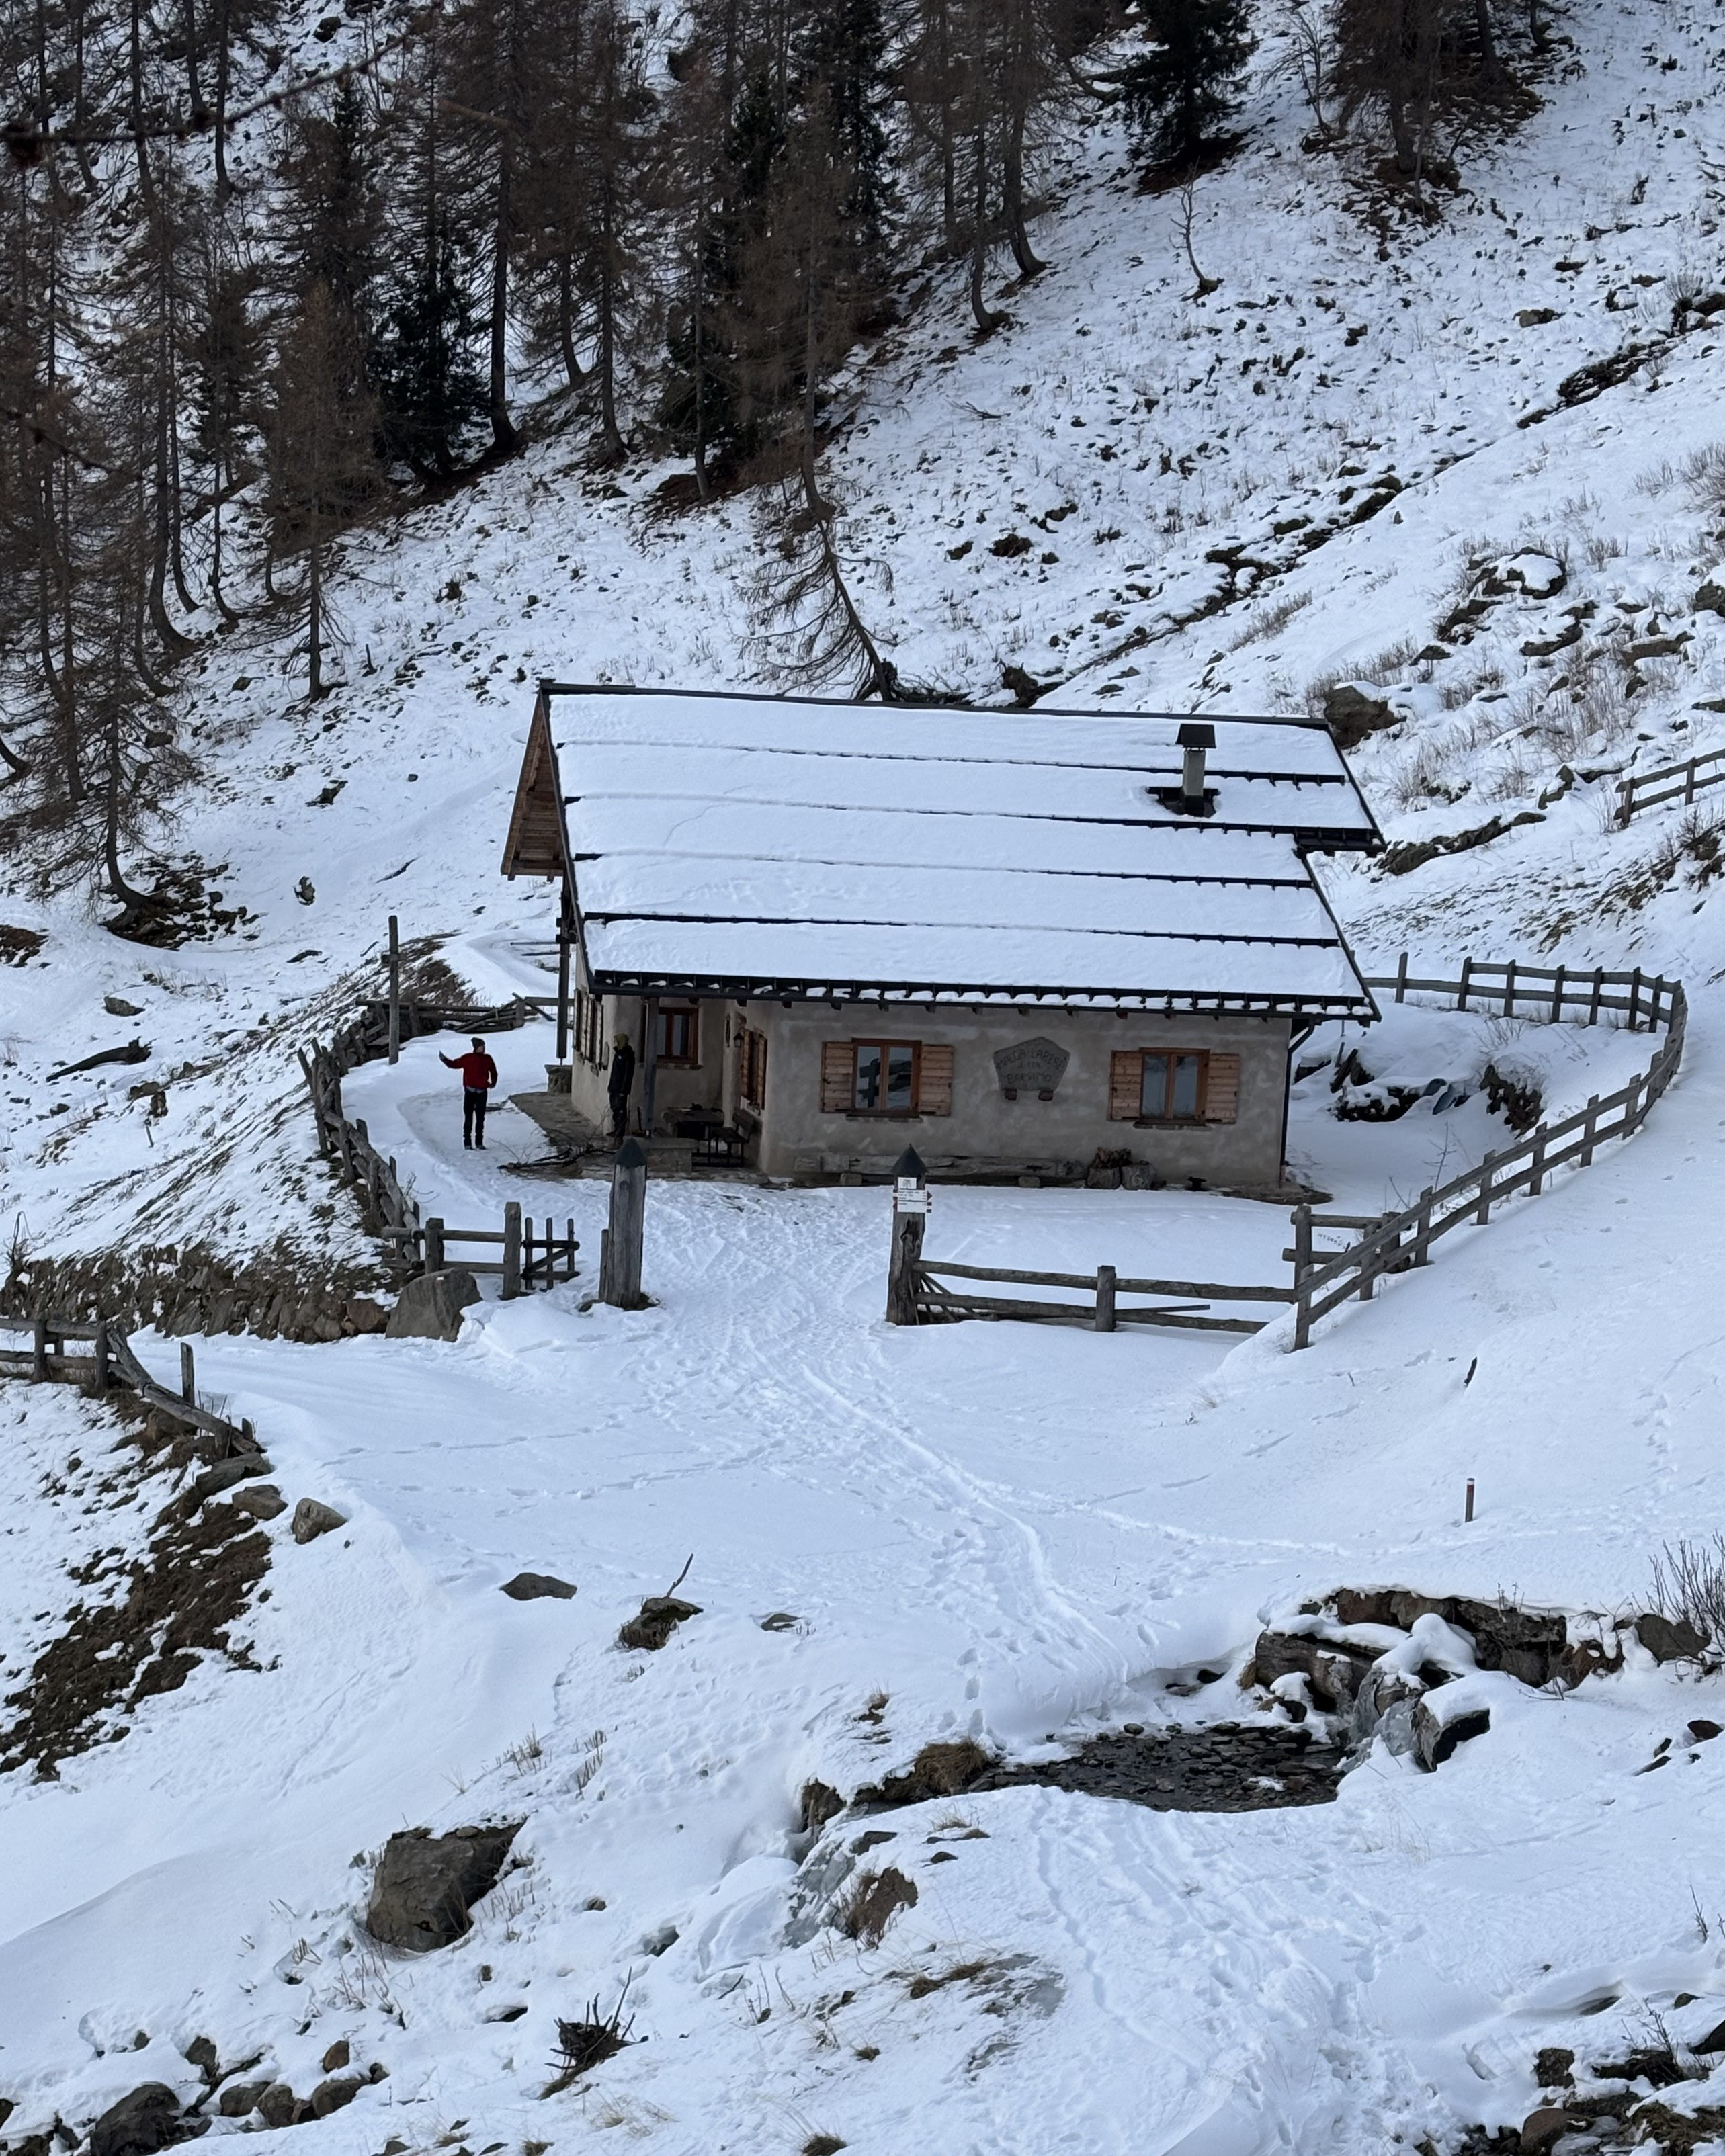
\includegraphics[width=\linewidth]{images/bivacco.jpeg}
\end{minipage}%
\hfill
\begin{minipage}[t]{0.5\textwidth}
  \vspace{0pt} % forza l'allineamento in alto
  
  Gruppo montuoso\\
  \textbf{\large Catena delle Maddalene}
  \\[1em] % Aggiunge una riga vuota qui
  Località\\
  \textbf{\large Bresimo, Val di Non}
  \\[1em] % Aggiunge una riga vuota qui
  Comune\\  
  \textbf{\large Bresimo}
  \\[1em] % Aggiunge una riga vuota qui
  Altezza\\  
  \textbf{\large 1774 m s.l.m.}
  \\[1em] % Aggiunge una riga vuota qui
  Apertura\\  
  \textbf{\large Gestito da Azienda agricola Giancarlo Carbonari, sempre aperto}

\end{minipage}

\subsection{Caratteristiche}
Il Bivacco Malga Laresè di sotto (bassa) è una struttura unica composta da stalla, alloggio per il pastore (casara), e  bivacco. È fornito di energia elettrica, acqua calda, solo nel periodo di apertura.

Il bivacco è suddiviso su due piani:
\begin{itemize}
    \item \textbf{Piano terra}: spazio principale della malga, un ampia stanza con tavolo, panche, stufa a legna, lavandino e dispensa con diverso materiale (bombole, candele, acqua, risotti, giochi da tavolo, ecc.).
    \item \textbf{Piano superiore}: diviso in diverse stanze, con un totale di circa 20 brande con materasso. \'E presente anche un bagno con lavandino e water (ne sconsiglio l'utilizzo per mancanza di acqua nel periodo di chiusura).
    \item \textbf{Spazio esterno}: si presenta una stalla molto ampia e dietro al bivacco si può trovare una legnaia al tempo ben fornita. Il bivacco è poi "circondato" dal passaggio di 2 corsi d'acqua non molto grandi.
\end{itemize}

Sebbene sia presente una legniaia è comunque semplice ricavare la legna grazie al bosco che circonda il bivacco.

La vista dalla malga è spettacolare, si riesce ad osservare tutta la vallata... E di notte quando il sole cala si crea uno spettacolo luminoso incredibile tra le vie valle e il cielo stellato.

\section{Come ci siamo arrivati}
Mi piacerebbe dire che questa era la meta che ci eravamo preposti ma così non è. Il nostro obiettivo era raggiungere il bivacco Pozze, poco più in su. Tuttavia, per colpa dell'ora tarda e della stanchezza generale, ci siamo dovuti fermare a questo bivacco.
Siamo arrivati al punto di partenza verso le 13.00 e la salita al bivacco è stata complessa. Il periodo invernale (siamo saliti il 31 dicembre per festeggiare capodanno insieme) non ha aiutato, era presente molta neve sul percorso al punto che senza ciaspole si sprofondava fino al ginocchio. Il giorno successivo abbiamo poi deciso di fare la stessa strada per tornare indietro.

Lascio comunque i dati del giro completo che avevamo intenzione di fare, anche se poi è andata diversamente.

\begin{figure}[htbp!]
    \centering
    % Colonna di sinistra, allineata in alto
    \begin{subfigure}[t]{0.45\textwidth}
        \centering
        \vspace{0pt} % Forziamo l'allineamento in alto
        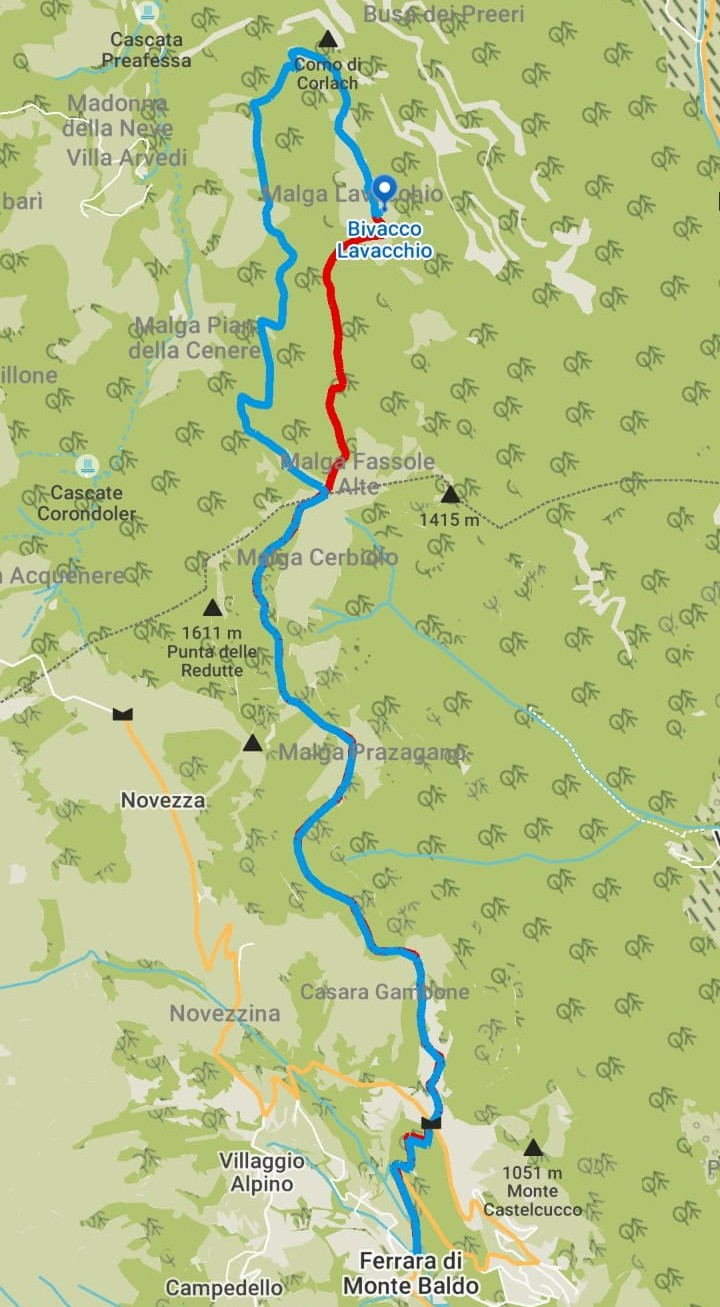
\includegraphics[width=\textwidth]{images/sentiero_mapsMe.jpg}
        \caption{Sentiero su Maps.Me.}
        \label{fig:foto_lunga}
    \end{subfigure}
    \hfill
    % Colonna di destra, allineata in alto
    \begin{subfigure}[t]{0.45\textwidth}
        \centering
        \vspace{0pt} % Forziamo l'allineamento in alto anche qui
        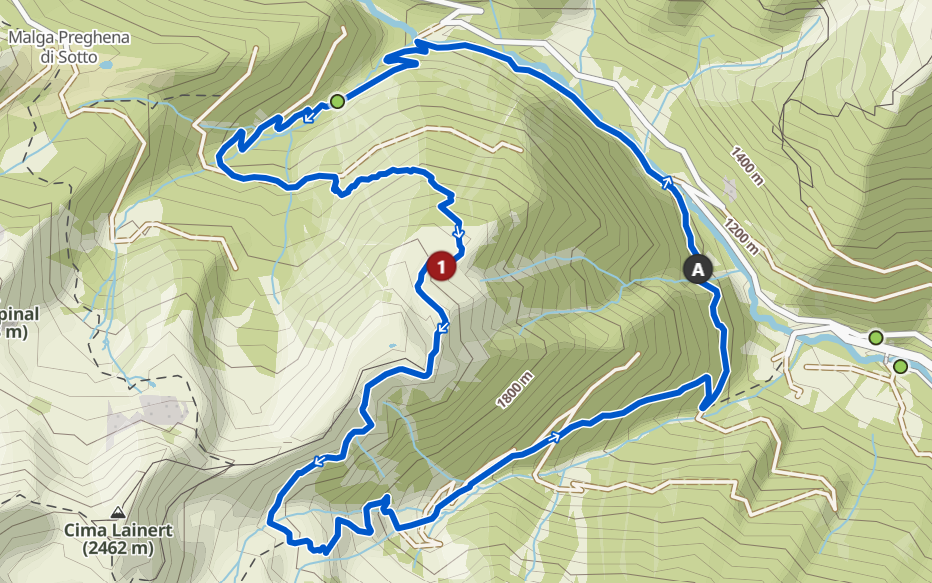
\includegraphics[width=\textwidth]{images/sentiero_komoot.png}
        \caption{Sentiero su Komoot.}
        \label{fig:foto_corta1}
        \vspace{1em} % Aggiunge un po' di spazio tra le due foto
        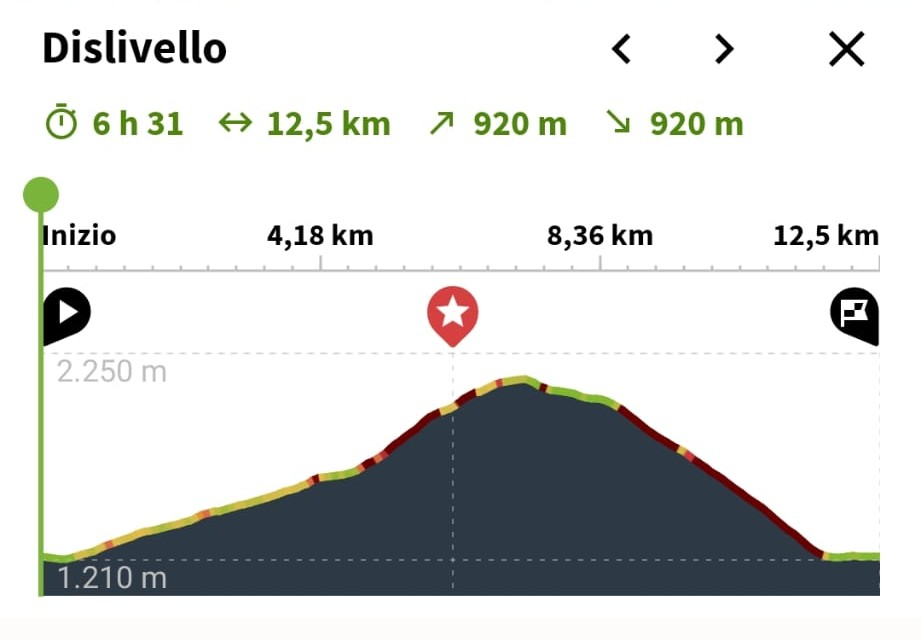
\includegraphics[width=\textwidth]{images/profilo_altimetrico.jpg}
        \caption{Profilo altimetrico del percorso.}
        \label{fig:foto_corta2}
    \end{subfigure}
    % Didascalia generale per l'intera figura
    \caption{Il sentiero e i dettagli del percorso.}
    \label{fig:panoramica_dettagli}
\end{figure}


\section{Non ti scordar di me}
\textbf{\textcolor{BurntOrange}{Ricorda: il bivacco è un bene comune. Il suo futuro dipende dal rispetto e dal senso civico dei visitatori. Usalo con cura e lascialo più pulito di come l'hai trovato.}}


\section{Alcune foto}

\begin{figure}[htbp!]
    \centering
    % Prima immagine
    \begin{subfigure}[b]{0.45\textwidth}
        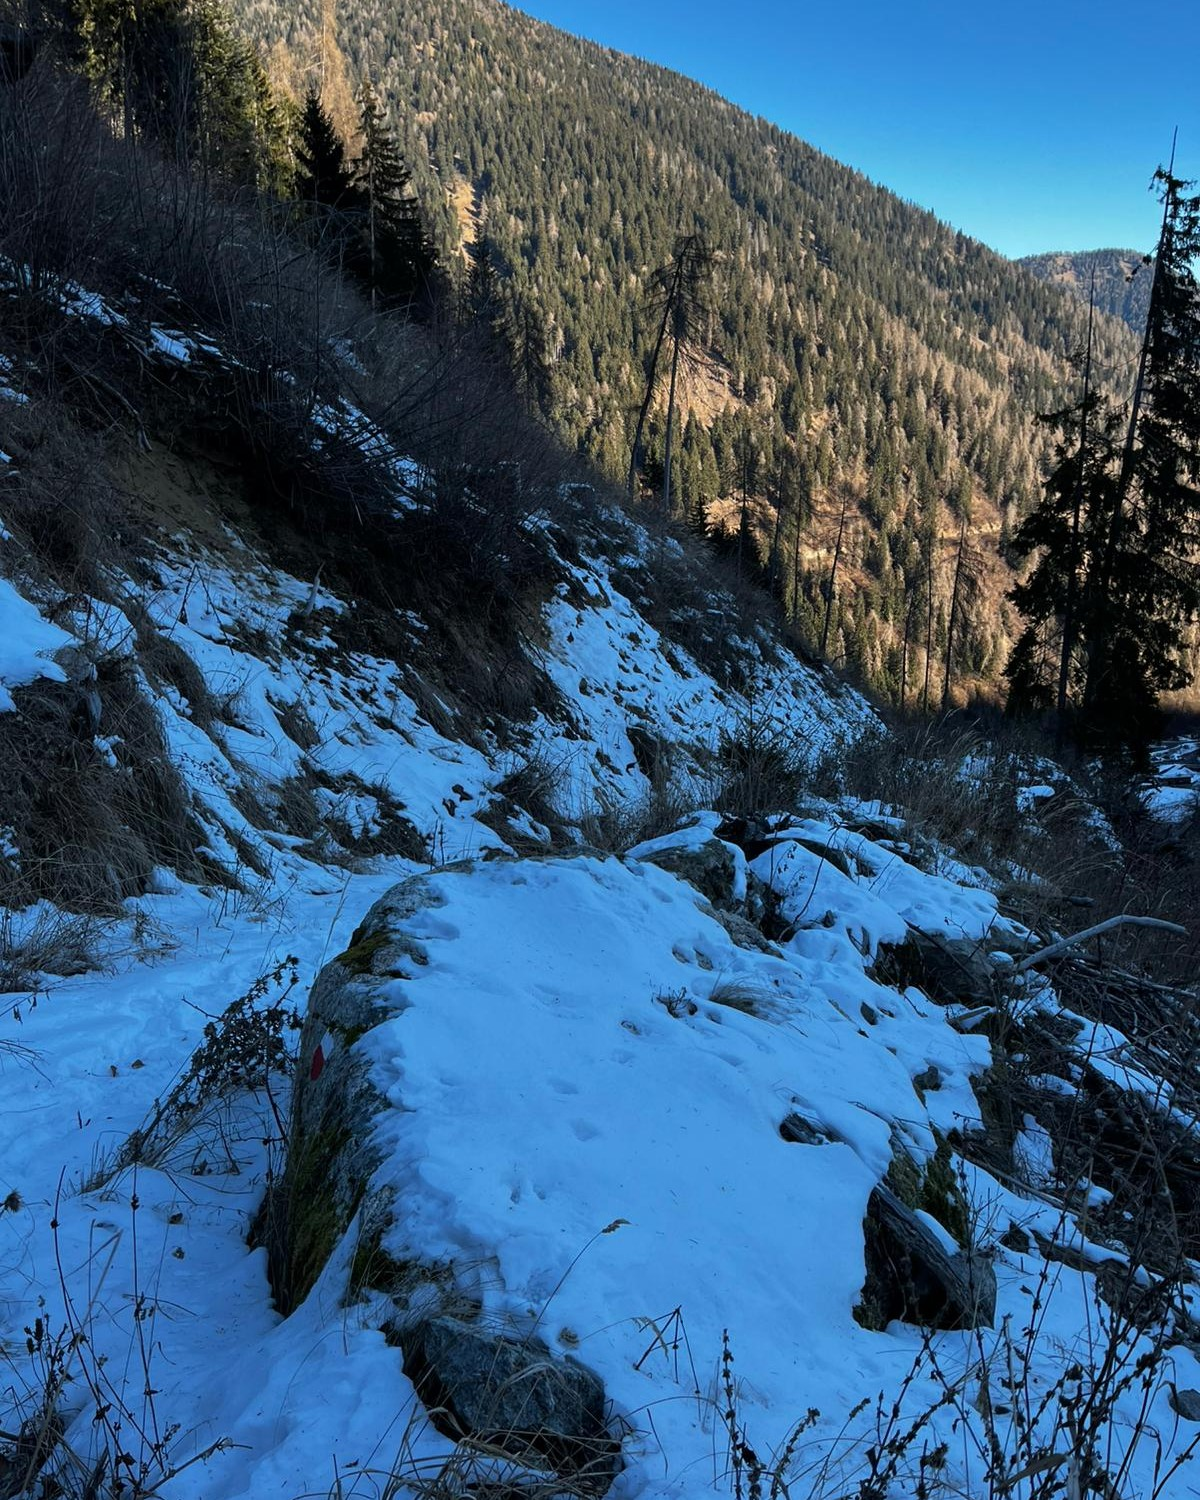
\includegraphics[width=\textwidth]{images/foto_sentiero.jpg}
        \caption{Sentiero.}
        \label{fig:prima_foto}
    \end{subfigure}
    \hfill
    % Seconda immagine
    \begin{subfigure}[b]{0.45\textwidth}
        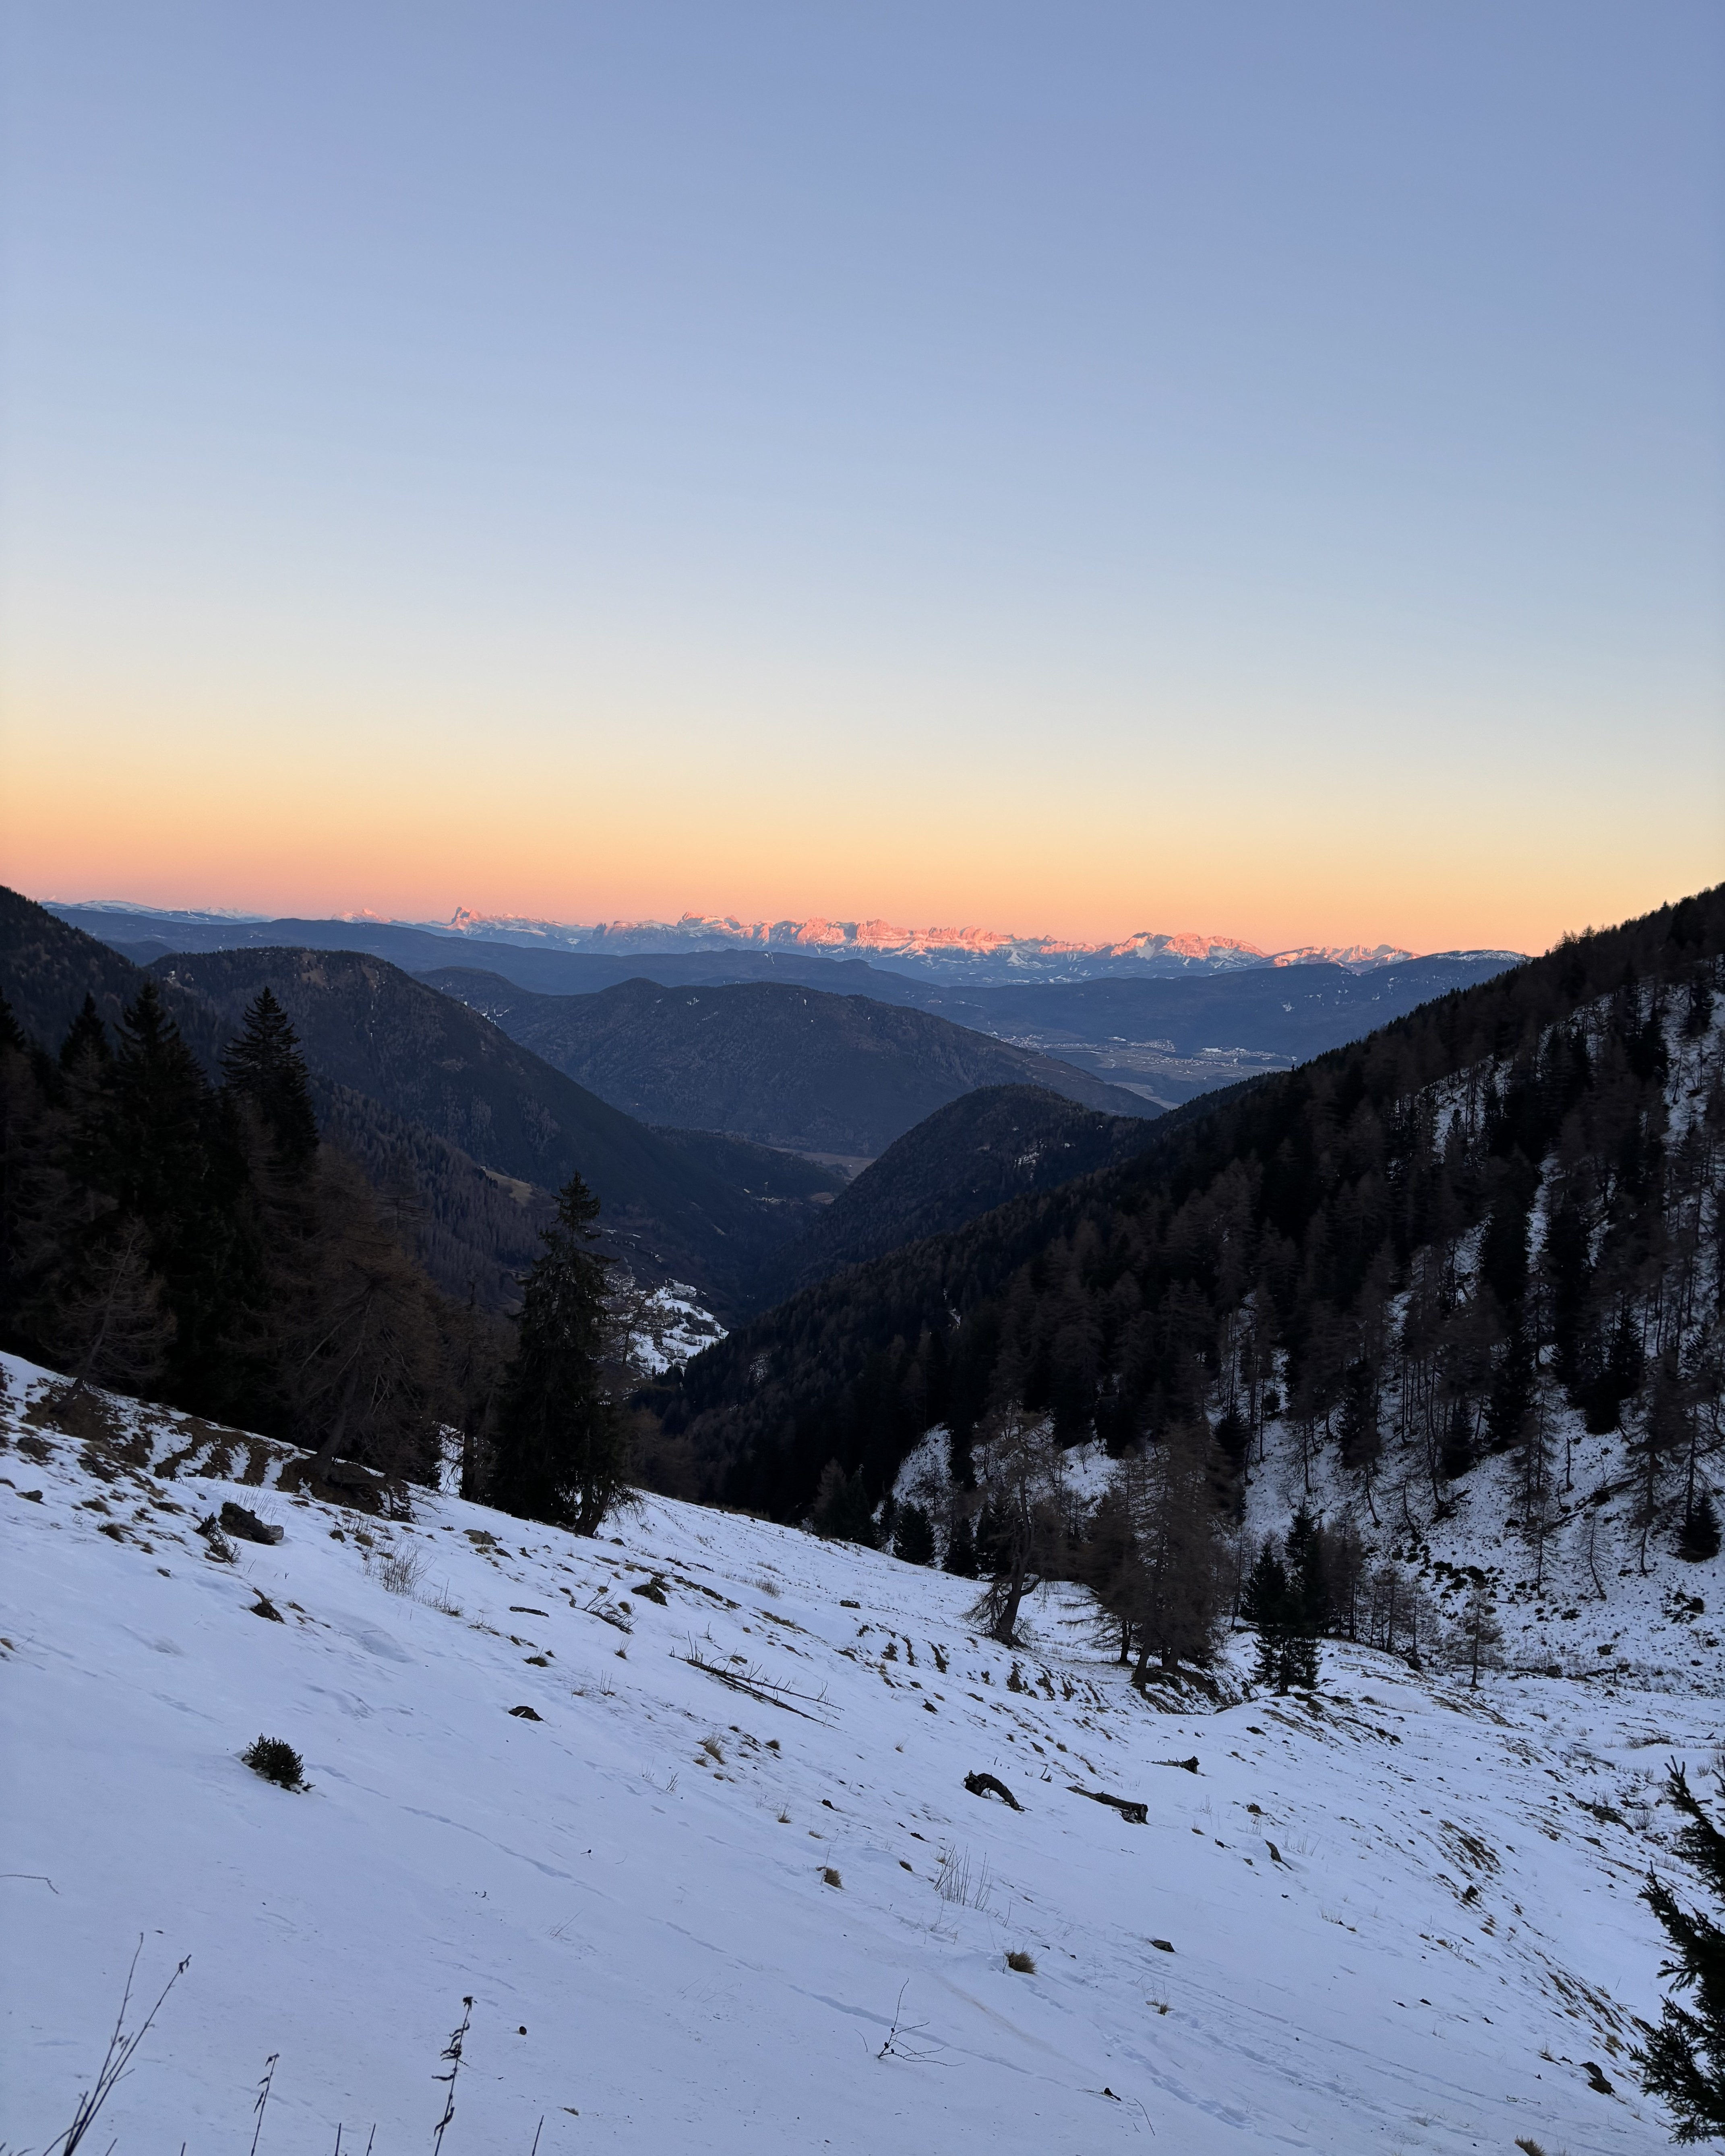
\includegraphics[width=\textwidth]{images/foto_paesaggio.jpeg}
        \caption{Vista dal bivacco.}
        \label{fig:seconda_foto}
    \end{subfigure}

    \vspace{1em} % Aggiunge un po' di spazio tra la riga sopra e la foto sotto
    % Terza immagine sotto
    \begin{subfigure}[b]{0.9\textwidth}
        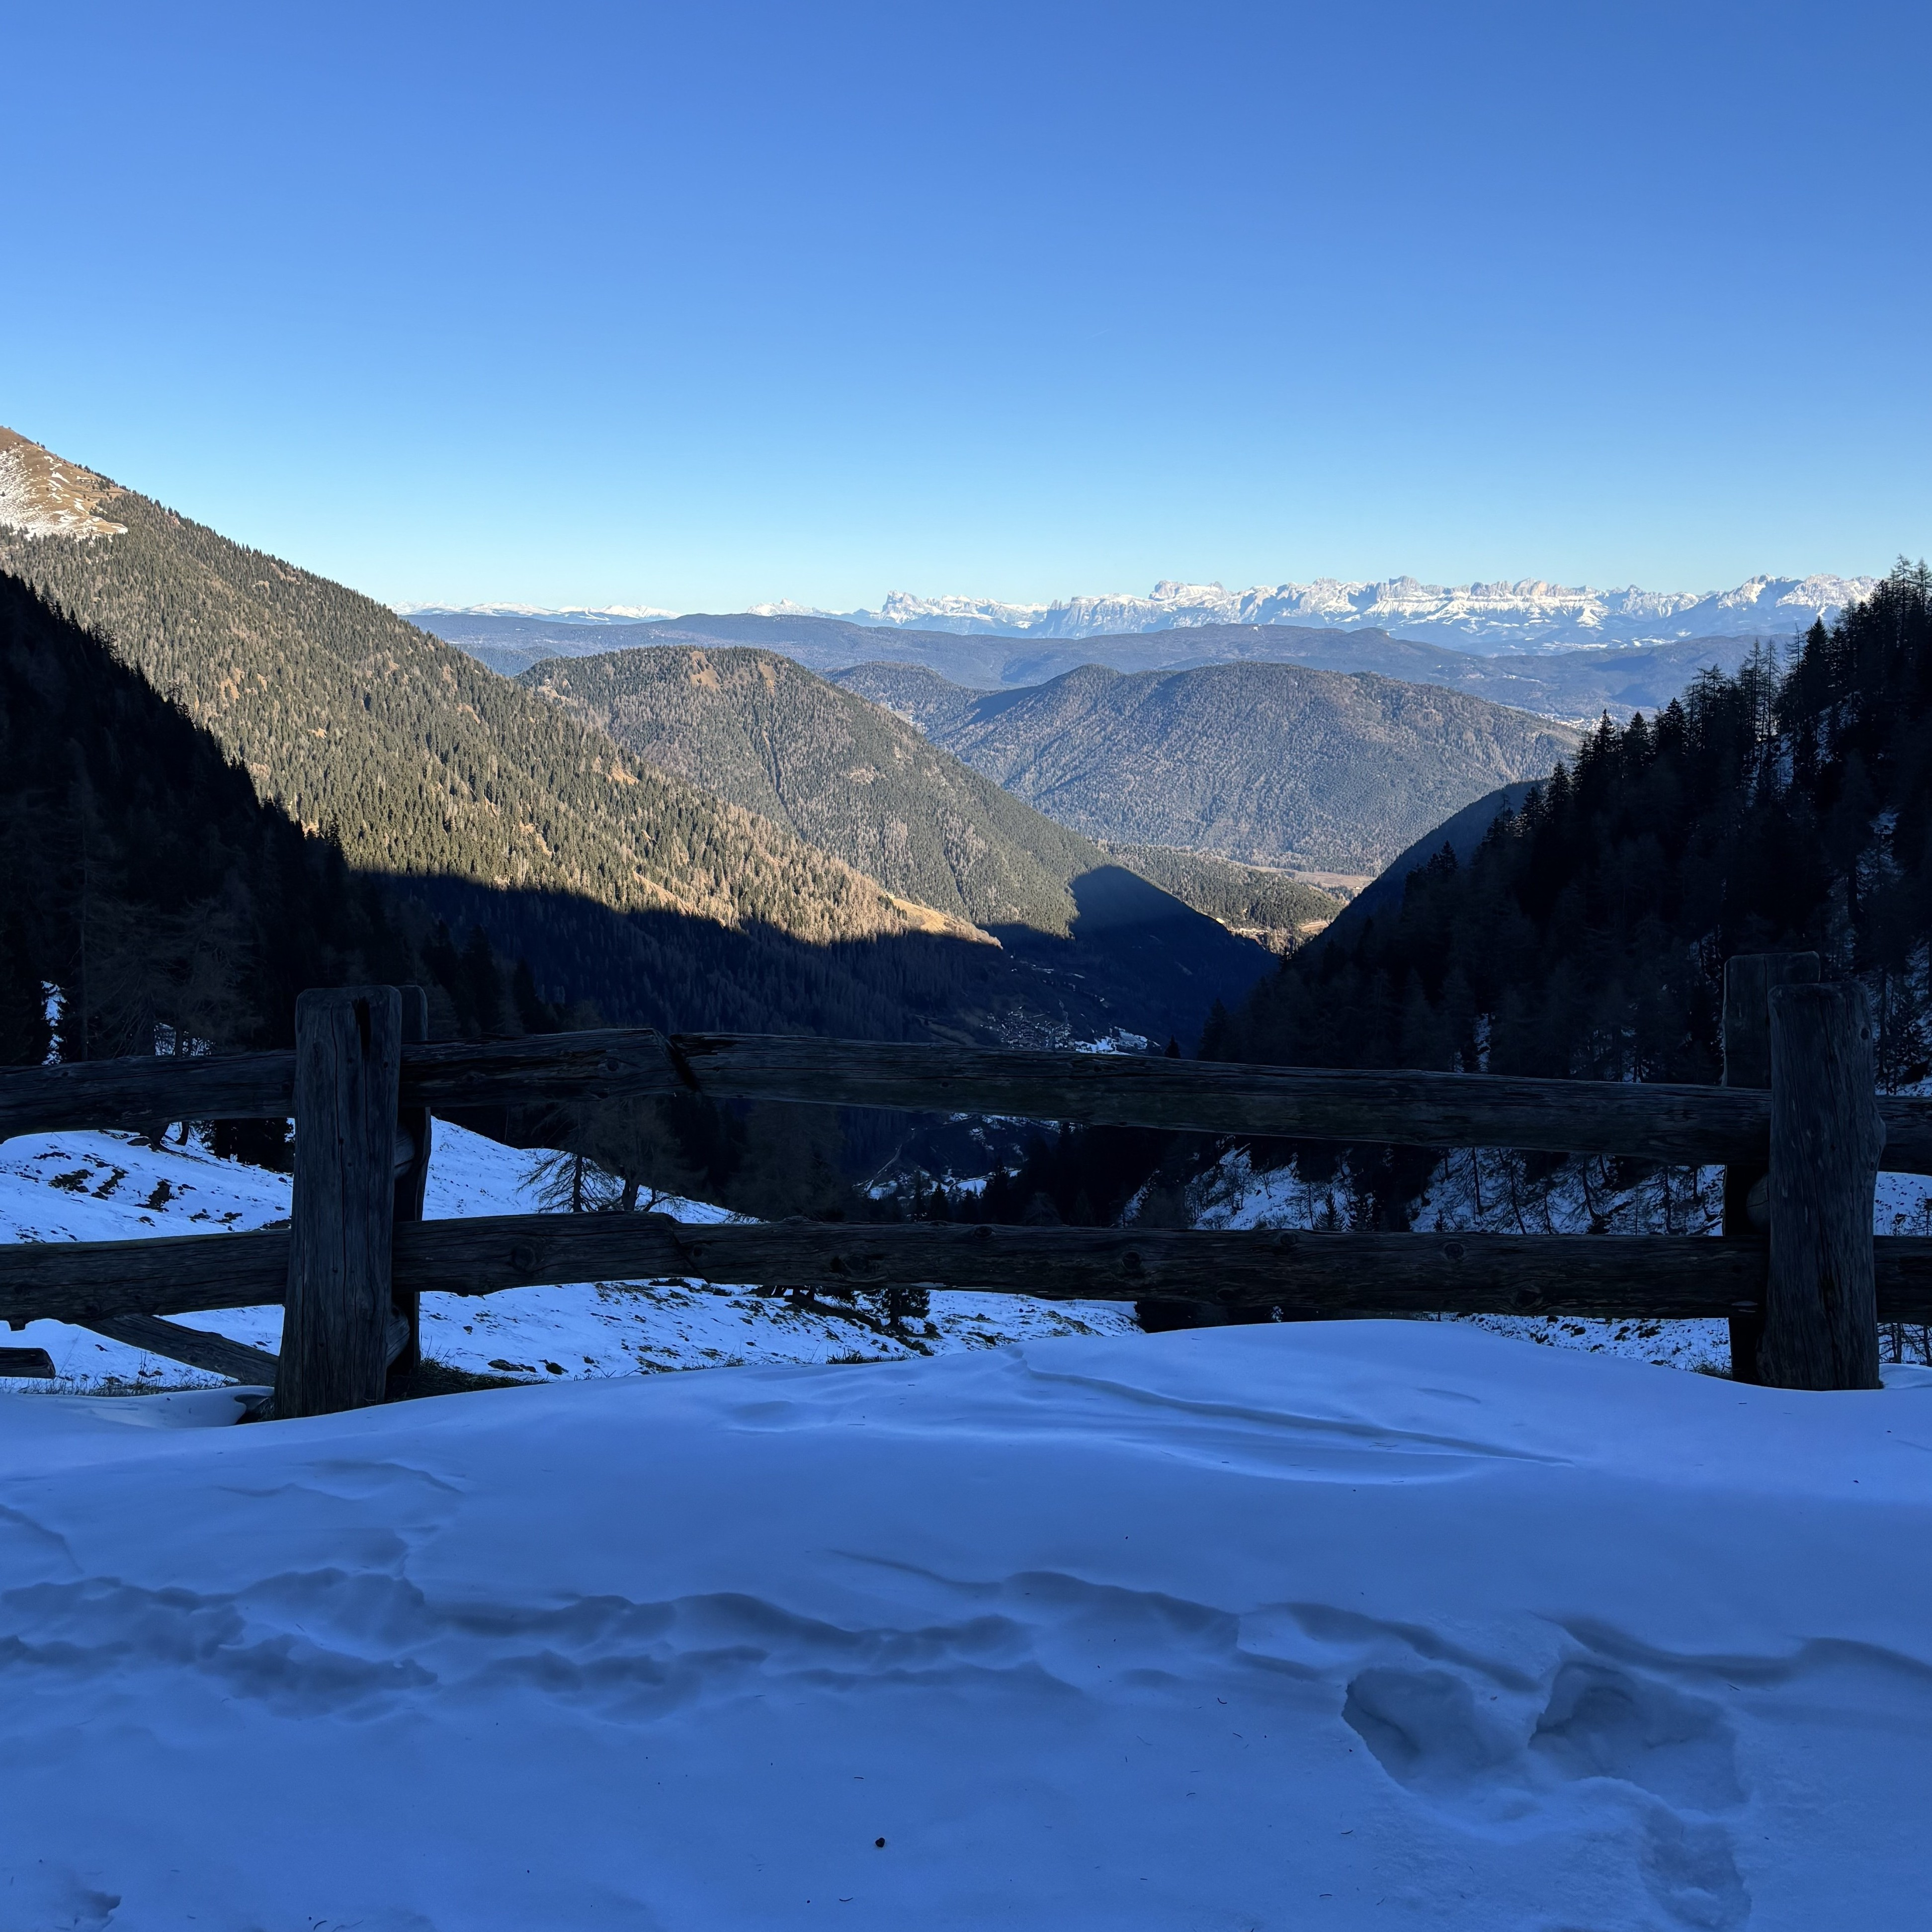
\includegraphics[width=\textwidth]{images/foto_vista.jpeg}
        \caption{Panoramica.}
        \label{fig:terza_foto}
    \end{subfigure}
    \caption{Selezione di fotografie del percorso e della vista dal bivacco.}
    \label{fig:foto}
\end{figure}

\end{document}
